% Options for packages loaded elsewhere
\PassOptionsToPackage{unicode}{hyperref}
\PassOptionsToPackage{hyphens}{url}
%
\documentclass[
]{book}
\usepackage{amsmath,amssymb}
\usepackage{lmodern}
\usepackage{iftex}
\ifPDFTeX
  \usepackage[T1]{fontenc}
  \usepackage[utf8]{inputenc}
  \usepackage{textcomp} % provide euro and other symbols
\else % if luatex or xetex
  \usepackage{unicode-math}
  \defaultfontfeatures{Scale=MatchLowercase}
  \defaultfontfeatures[\rmfamily]{Ligatures=TeX,Scale=1}
\fi
% Use upquote if available, for straight quotes in verbatim environments
\IfFileExists{upquote.sty}{\usepackage{upquote}}{}
\IfFileExists{microtype.sty}{% use microtype if available
  \usepackage[]{microtype}
  \UseMicrotypeSet[protrusion]{basicmath} % disable protrusion for tt fonts
}{}
\makeatletter
\@ifundefined{KOMAClassName}{% if non-KOMA class
  \IfFileExists{parskip.sty}{%
    \usepackage{parskip}
  }{% else
    \setlength{\parindent}{0pt}
    \setlength{\parskip}{6pt plus 2pt minus 1pt}}
}{% if KOMA class
  \KOMAoptions{parskip=half}}
\makeatother
\usepackage{xcolor}
\usepackage{color}
\usepackage{fancyvrb}
\newcommand{\VerbBar}{|}
\newcommand{\VERB}{\Verb[commandchars=\\\{\}]}
\DefineVerbatimEnvironment{Highlighting}{Verbatim}{commandchars=\\\{\}}
% Add ',fontsize=\small' for more characters per line
\usepackage{framed}
\definecolor{shadecolor}{RGB}{248,248,248}
\newenvironment{Shaded}{\begin{snugshade}}{\end{snugshade}}
\newcommand{\AlertTok}[1]{\textcolor[rgb]{0.94,0.16,0.16}{#1}}
\newcommand{\AnnotationTok}[1]{\textcolor[rgb]{0.56,0.35,0.01}{\textbf{\textit{#1}}}}
\newcommand{\AttributeTok}[1]{\textcolor[rgb]{0.77,0.63,0.00}{#1}}
\newcommand{\BaseNTok}[1]{\textcolor[rgb]{0.00,0.00,0.81}{#1}}
\newcommand{\BuiltInTok}[1]{#1}
\newcommand{\CharTok}[1]{\textcolor[rgb]{0.31,0.60,0.02}{#1}}
\newcommand{\CommentTok}[1]{\textcolor[rgb]{0.56,0.35,0.01}{\textit{#1}}}
\newcommand{\CommentVarTok}[1]{\textcolor[rgb]{0.56,0.35,0.01}{\textbf{\textit{#1}}}}
\newcommand{\ConstantTok}[1]{\textcolor[rgb]{0.00,0.00,0.00}{#1}}
\newcommand{\ControlFlowTok}[1]{\textcolor[rgb]{0.13,0.29,0.53}{\textbf{#1}}}
\newcommand{\DataTypeTok}[1]{\textcolor[rgb]{0.13,0.29,0.53}{#1}}
\newcommand{\DecValTok}[1]{\textcolor[rgb]{0.00,0.00,0.81}{#1}}
\newcommand{\DocumentationTok}[1]{\textcolor[rgb]{0.56,0.35,0.01}{\textbf{\textit{#1}}}}
\newcommand{\ErrorTok}[1]{\textcolor[rgb]{0.64,0.00,0.00}{\textbf{#1}}}
\newcommand{\ExtensionTok}[1]{#1}
\newcommand{\FloatTok}[1]{\textcolor[rgb]{0.00,0.00,0.81}{#1}}
\newcommand{\FunctionTok}[1]{\textcolor[rgb]{0.00,0.00,0.00}{#1}}
\newcommand{\ImportTok}[1]{#1}
\newcommand{\InformationTok}[1]{\textcolor[rgb]{0.56,0.35,0.01}{\textbf{\textit{#1}}}}
\newcommand{\KeywordTok}[1]{\textcolor[rgb]{0.13,0.29,0.53}{\textbf{#1}}}
\newcommand{\NormalTok}[1]{#1}
\newcommand{\OperatorTok}[1]{\textcolor[rgb]{0.81,0.36,0.00}{\textbf{#1}}}
\newcommand{\OtherTok}[1]{\textcolor[rgb]{0.56,0.35,0.01}{#1}}
\newcommand{\PreprocessorTok}[1]{\textcolor[rgb]{0.56,0.35,0.01}{\textit{#1}}}
\newcommand{\RegionMarkerTok}[1]{#1}
\newcommand{\SpecialCharTok}[1]{\textcolor[rgb]{0.00,0.00,0.00}{#1}}
\newcommand{\SpecialStringTok}[1]{\textcolor[rgb]{0.31,0.60,0.02}{#1}}
\newcommand{\StringTok}[1]{\textcolor[rgb]{0.31,0.60,0.02}{#1}}
\newcommand{\VariableTok}[1]{\textcolor[rgb]{0.00,0.00,0.00}{#1}}
\newcommand{\VerbatimStringTok}[1]{\textcolor[rgb]{0.31,0.60,0.02}{#1}}
\newcommand{\WarningTok}[1]{\textcolor[rgb]{0.56,0.35,0.01}{\textbf{\textit{#1}}}}
\usepackage{longtable,booktabs,array}
\usepackage{calc} % for calculating minipage widths
% Correct order of tables after \paragraph or \subparagraph
\usepackage{etoolbox}
\makeatletter
\patchcmd\longtable{\par}{\if@noskipsec\mbox{}\fi\par}{}{}
\makeatother
% Allow footnotes in longtable head/foot
\IfFileExists{footnotehyper.sty}{\usepackage{footnotehyper}}{\usepackage{footnote}}
\makesavenoteenv{longtable}
\usepackage{graphicx}
\makeatletter
\def\maxwidth{\ifdim\Gin@nat@width>\linewidth\linewidth\else\Gin@nat@width\fi}
\def\maxheight{\ifdim\Gin@nat@height>\textheight\textheight\else\Gin@nat@height\fi}
\makeatother
% Scale images if necessary, so that they will not overflow the page
% margins by default, and it is still possible to overwrite the defaults
% using explicit options in \includegraphics[width, height, ...]{}
\setkeys{Gin}{width=\maxwidth,height=\maxheight,keepaspectratio}
% Set default figure placement to htbp
\makeatletter
\def\fps@figure{htbp}
\makeatother
\setlength{\emergencystretch}{3em} % prevent overfull lines
\providecommand{\tightlist}{%
  \setlength{\itemsep}{0pt}\setlength{\parskip}{0pt}}
\setcounter{secnumdepth}{5}
\usepackage{booktabs}
\usepackage{amsthm}
\makeatletter
\def\thm@space@setup{%
  \thm@preskip=8pt plus 2pt minus 4pt
  \thm@postskip=\thm@preskip
}
\makeatother
\ifLuaTeX
  \usepackage{selnolig}  % disable illegal ligatures
\fi
\usepackage[]{natbib}
\bibliographystyle{apalike}
\IfFileExists{bookmark.sty}{\usepackage{bookmark}}{\usepackage{hyperref}}
\IfFileExists{xurl.sty}{\usepackage{xurl}}{} % add URL line breaks if available
\urlstyle{same} % disable monospaced font for URLs
\hypersetup{
  pdftitle={Lab Handbook},
  pdfauthor={Bram Kuijper},
  hidelinks,
  pdfcreator={LaTeX via pandoc}}

\title{Lab Handbook}
\author{Bram Kuijper}
\date{2022-06-16}

\begin{document}
\maketitle

{
\setcounter{tocdepth}{1}
\tableofcontents
}
\hypertarget{introduction}{%
\chapter{Introduction}\label{introduction}}

This document gives you an overview of some of the key computing practices used in our lab. Enjoy!

\hypertarget{installing-and-using-software-to-do-your-work}{%
\chapter{Installing and using software to do your work}\label{installing-and-using-software-to-do-your-work}}

To do your research in theoretical or computational biology, you will need to install a bunch of software. I typically try to keep things as free and open access as possible, so that you don't have hassle with license fees. However, this is not always possible (e.g., research projects involving Mathematica or matlab).

\hypertarget{finding-out-what-software-you-need}{%
\section{Finding out what software you need}\label{finding-out-what-software-you-need}}

Don't install \emph{all} the software listed below. Rather contact me to discuss what software you need. Typically, you need one (or two) of the following options:

\begin{enumerate}
\def\labelenumi{\arabic{enumi}.}
\tightlist
\item
  The Rstudio environment
\item
  A Python environment
\item
  A C++ environment
\item
  A Mathematica environment
\end{enumerate}

\hypertarget{the-rstudio-environment}{%
\section{The Rstudio environment}\label{the-rstudio-environment}}

R is a very commonly used programming environment and particularly useful for data analysis. Its disadvantages are that it is slow and that the programming language is arcane, to say the least. All pros and cons considered, if your project is data heavy, R is a great choice.

Rather than using the \href{https://cran.r-project.org/}{absolute bare bones version of the programming environment R}, we use \href{https://www.rstudio.com/}{Rstudio}, because it provides a full-blown IDE (integrated development environment) with text editor, variable inspector, file browswer and more. You can either use your web browser to go to the online \href{https://rstudio01.cles.ex.ac.uk}{Rstudio server} that is offered by the University of Exeter. Alternatively, you can choose to use a locally installed version of Rstudio (see below for installation instructions). If you don't know whether to choose the server-based version or the local installed he server-based version of Rstudio is probably the easiest to use, as it already has tons of packages pre-installed. However, if you have no uni access anymore or don't have continuous internet access, a locally installed version of Rstudio is best.

\hypertarget{installing-rstudio-on-a-mac}{%
\subsection{Installing Rstudio on a mac}\label{installing-rstudio-on-a-mac}}

A great way of keeping Rstudio up-to-date is to first install the Homebrew package manager
\href{https://brew.sh}{Homebrew}. This is a small program that allows you to install and update multiple programs on your Mac. Indeed, almost any research software that you will need on your Mac can be installed with homebrew. Using homebrew has the advantage that installation involves a single command, rather than you having to search for the correct version of the software online. Moreover, all installed packages will be updated to their latest versions by using two simple commands: \texttt{brew\ update}, following by \texttt{brew\ upgrade}.

\hypertarget{installing-homebrew}{%
\subsection{Installing homebrew}\label{installing-homebrew}}

To install homebrew, you need to open the Terminal app (see \protect\hyperlink{MacTerminal}{here} about where to find the Terminal app on your Mac). Once the terminal is open, copy the single-line install statement from the \href{https://brew.sh/}{Homebrew website} and paste it into the Terminal app. Then press `Enter'. You will get a bunch of straightforward questions, after which homebrew installs itself.

\hypertarget{installing-your-first-application-using-homebrew}{%
\subsection{Installing your first application using homebrew}\label{installing-your-first-application-using-homebrew}}

After homebrew is installed, you can use it to install other applications. You can search for software available for install through homebrew by using the website \href{https://formulae.brew.sh}{formulae.brew.sh}.

Let us install the {[}Textmate{]} text editor that we might need later. We do so using the \protect\hyperlink{MacTerminal}{Terminal app} app, in which we type

\begin{Shaded}
\begin{Highlighting}[]
\ExtensionTok{brew}\NormalTok{ install }\AttributeTok{{-}{-}cask}\NormalTok{ textmate}
\end{Highlighting}
\end{Shaded}

\hypertarget{updating-all-applications-that-have-been-installed-via-homebrew}{%
\subsection{Updating all applications that have been installed via homebrew}\label{updating-all-applications-that-have-been-installed-via-homebrew}}

This is where things get handier than installing all software individually:

\begin{Shaded}
\begin{Highlighting}[]
\ExtensionTok{brew}\NormalTok{ update }\KeywordTok{\&\&} \ExtensionTok{brew}\NormalTok{ upgrade}
\end{Highlighting}
\end{Shaded}

\hypertarget{rstudio}{%
\section{Rstudio}\label{rstudio}}

\hypertarget{using-the-web-based-rstudio-server}{%
\subsection{Using the web-based Rstudio server}\label{using-the-web-based-rstudio-server}}

You can simply access this by using your web browser. You can access the Rstudio server here:
\url{https://rstudio01.cles.ex.ac.uk}, using your University of Exeter login.

Once logged in, make sure to run the 4.x.x version, rather than a 3.x.x version. You can change versions on the top right of your Rstudio window within in your web browser. See the image below

\hypertarget{installing-rstudio-on-your-own-computer-on-windows-or-mac}{%
\subsection{Installing Rstudio on your own computer on windows or mac}\label{installing-rstudio-on-your-own-computer-on-windows-or-mac}}

If you have a Windows machine, the best way to install Rstudio is to download the \href{https://www.rstudio.com/products/rstudio/download/}{Desktop version}. If you are on a mac, one could use:

\begin{Shaded}
\begin{Highlighting}[]
\ExtensionTok{brew}\NormalTok{ install }\AttributeTok{{-}{-}cask}\NormalTok{ rstudio}
\end{Highlighting}
\end{Shaded}

\hypertarget{installing-python}{%
\section{Installing Python}\label{installing-python}}

For those of you who will need to install python (installing python is more the exception than the norm, hence ask if unsure), it is best to install the \href{https://www.anaconda.com/products/individual}{Anaconda} distribution, which provides the whole python bundle and comes with a package manager.

\hypertarget{section:mobaxterm}{%
\section{Windows: Accessing remote servers using mobaxterm}\label{section:mobaxterm}}

For some projects we need to access a remote server to run our software. For this we use the programme \href{https://mobaxterm.mobatek.net/download.html}{mobaxterm}.

To install mobaxterm, watch this handy \href{https://www.youtube.com/watch?v=KRpgYS-eHj8\&t=87s}{video}. Make sure you download the `Portable version' rather than the `Installer' version.

The mobaxterm-xxx.exe file can be ran from anywhere on your operating system (hence, the name Portable). Hence, try to put in a location where you will not forget it. Alternatively make a shortcut to the mobaxterm-xxx.exe file (Right mouse click \textgreater{} create shortcut) and then drag the shortcut to the taskbar in Windows. See \href{https://www.youtube.com/watch?v=3K9oYys-tYE}{this video} of some dude explaining everything taskbar-related on windows.

\hypertarget{using-mobaxterm-to-access-a-remote-location}{%
\subsection{Using Mobaxterm to access a remote location}\label{using-mobaxterm-to-access-a-remote-location}}

Now let's use mobaxterm to access the remote server.
\#\# Installing software to develop C++ programs \{\#section:installcpp\}
When working with the programming language C++, we will need to use the following software:

\begin{enumerate}
\def\labelenumi{\arabic{enumi}.}
\tightlist
\item
  A UNIX Terminal (already installed on a mac, you will need to install on windows - see below)
\item
  A C++ compiler, which in our case will be \texttt{clang} on mac and \texttt{g++} on windows (see below).
\item
  A better-than-normal text editor. When on Windows, install the freely available text editor \href{}{Notepad++}. See the Notepad++ website for installation instructions. When on a mac, install an editor such as textmate (see below).
\item
  A software build environment like make or cmake.
\end{enumerate}

\hypertarget{yes-we-really-need-a-unix-terminal.}{%
\section{Yes, we really need a UNIX terminal.}\label{yes-we-really-need-a-unix-terminal.}}

You will need a UNIX terminal to access a broad collection of tools, namely the compiler \texttt{g++} o turn your C++ code into an executable programme, the command \texttt{git} to get code from repositories and \texttt{make} or \texttt{cmake} to automate the building of your code.

Sure, it would be possible to avoid a UNIX toolchain, by using Microsoft's Visual Studio or another compiler. However, chances are that we'll be running things on one of the University's Linux \href{https://universityofexeteruk.sharepoint.com/sites/CornwallARC}{computing clusters} later on. If one has been working with Visual Studio, it typically is a massive pain to switch back to the different tools and compilers used on these Linux clusters, particularly when we would use associated libraries such as \texttt{gsl} or \texttt{eigen}. By contrast, when you already use a UNIX terminal on your local computer, moving to use the University's Linux cluster is very easy.

\hypertarget{windows-install-msys2-as-our-unix-terminal}{%
\section{Windows: install MSYS2 as our UNIX terminal}\label{windows-install-msys2-as-our-unix-terminal}}

To get a UNIX terminal running on windows, we will install the \href{https://www.msys2.org/}{MSYS2} environment. See \href{https://recapexeter.cloud.panopto.eu/Panopto/Pages/Viewer.aspx?id=f2acdf3c-224e-49be-8ae3-ad2400f2b3c1\&start=0}{here} for the installation video. There is also \href{https://recapexeter.cloud.panopto.eu/Panopto/Pages/Viewer.aspx?id=376342e6-5791-4c25-b2e3-ad2400ffe304\&start=0}{another video} that shows you how to subsequently work with the compiler, once installed.

\hypertarget{accessing-msys2-once-installed}{%
\subsection{Accessing MSYS2 once installed}\label{accessing-msys2-once-installed}}

Once everything is installed, use the MSYS2 MinGW x64 executable, rather than the default MSYS2 executable. To start this, simply type \texttt{msys} in the windows search box (see screenshot) and the \texttt{x64} version will appear in the menu:

\begin{figure}
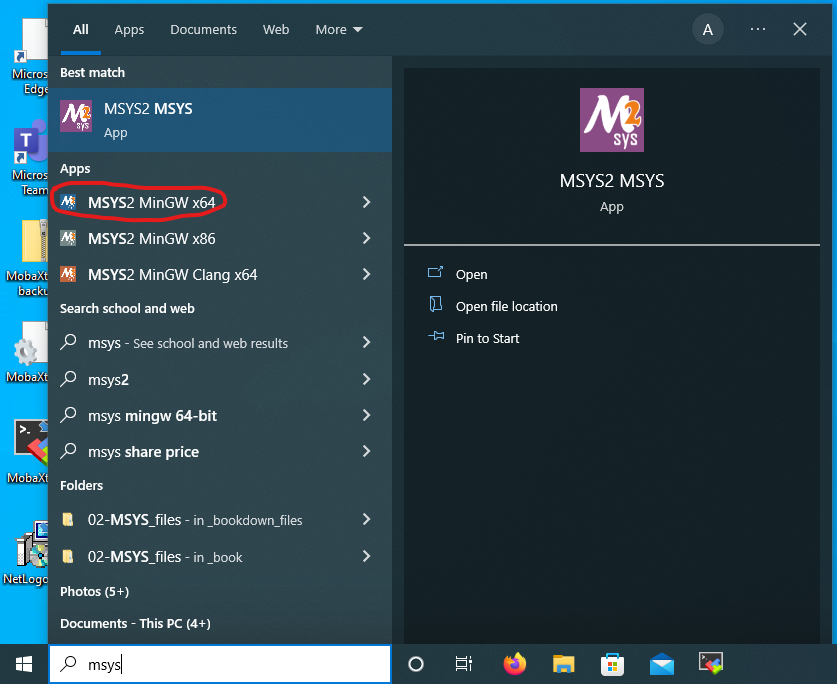
\includegraphics[width=11.62in]{images/screenshot_windows_msys64_menu} \caption{Location of MSYS x64 in the windows menu. The default MSYS2 app will appear on top, but the x64 version can be found right below (red circle).}\label{fig:figScreenShotMenu}
\end{figure}

\hypertarget{section:MSYS2homedir}{%
\subsection{Accessing MSYS2's home directory through Windows File Explorer}\label{section:MSYS2homedir}}

The home directory in MSYS2 is indicated by the \texttt{\textasciitilde{}} sign, which points to a directory on your hard drive. However, the MSYS2 home directory is not the same as your Windows home directory! Rather, MSYS2's home directory \texttt{\textasciitilde{}} maps to something like \texttt{C:/msys64/home/\$your\_user\_name}, rather than to the usual location of the windows home directory which is something like \texttt{C:/Users/\$your\_user\_name/home}, where you need to replace \texttt{\$your\_user\_name} with your windows user name.

Knowing that \texttt{\textasciitilde{}} is somewhere else than the standard home directory, you can still use the \href{https://support.microsoft.com/en-us/windows/find-and-open-file-explorer-ef370130-1cca-9dc5-e0df-2f7416fe1cb1\#WindowsVersion=Windows_10}{Windows File Explorer} to access this location and inspect the files present in \texttt{\textasciitilde{}}. Click the \texttt{This\ PC} in the left column of the Windows File Explorer and go to \texttt{C:/msys64/home/\$your\_user\_name}. Here an example screenshot to clarify matters:

\begin{figure}
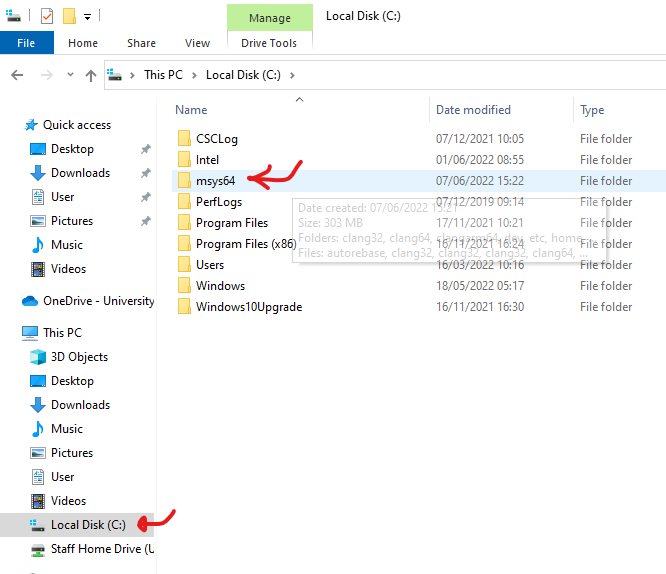
\includegraphics[width=500pt]{images/screenshot_windows_msys} \caption{Accessing the contents of the `msys64` directory via Windows File Explorer. Later on, the simulation code and simulation output will be found within this directory (in particular, within its `home` directory).}\label{fig:figWindowsExplorer}
\end{figure}

\hypertarget{installing-a-command-line-c-compiler-within-msys2}{%
\subsection{Installing a command-line C++ compiler within MSYS2}\label{installing-a-command-line-c-compiler-within-msys2}}

Rather than using any C++ compiler like Visual Studio or Code Blocks, we use the compiler \href{https://gcc.gnu.org/}{g++}, as that compiler is the same as used on our computing clusters. To install it, see the instruction video \href{https://recapexeter.cloud.panopto.eu/Panopto/Pages/Viewer.aspx?id=f2acdf3c-224e-49be-8ae3-ad2400f2b3c1\&start=0}{here}.

\hypertarget{installing-git-within-msys2}{%
\subsection{\texorpdfstring{Installing \texttt{git} within MSYS2}{Installing git within MSYS2}}\label{installing-git-within-msys2}}

We need \texttt{git} to download and synchronize code repositories. To install \texttt{git} within MSYS2 type the command

\begin{Shaded}
\begin{Highlighting}[]
\ExtensionTok{pacman} \AttributeTok{{-}S}\NormalTok{ git}
\end{Highlighting}
\end{Shaded}

\hypertarget{windows-use-notepad-as-your-text-editor-of-choice}{%
\subsection{Windows: use notepad++ as your text editor of choice}\label{windows-use-notepad-as-your-text-editor-of-choice}}

To edit and inspect source files, please \textbf{do not} use the standard text editor on windows, which is \href{https://apps.microsoft.com/store/detail/windows-notepad/9MSMLRH6LZF3?hl=en-us\&gl=US}{notepad}. This crippled and lame editor cannot read source files with line endings that are used on different operating systems like linux or mac. Moreover, it does not have syntax colouring, which is a life saver when reading code.

Hence, please install the free editor Notepad++ which provides syntax colouring and more.
You can download a copy of Notepad++ \href{https://notepad-plus-plus.org/downloads/}{here}.

If you don't like Notepad++, have a google yourself. Any code editor that supports syntax coloring of C++,R,Python files and supports \texttt{CR/LF} and \texttt{LF} line endings should be OK.

\hypertarget{mac-a-unix-terminal-is-provided-via-the-terminal-app-within-the-applicationsutilities-folder}{%
\section{Mac: a UNIX terminal is provided via the Terminal app within the Applications/Utilities folder}\label{mac-a-unix-terminal-is-provided-via-the-terminal-app-within-the-applicationsutilities-folder}}

To use the UNIX toolchain on a mac, you will need to use a UNIX terminal. Luckily this is installed as per default on any mac distribution. You can find the Terminal app in the \texttt{Applications} \textgreater{} \texttt{Utilities} folder on your hard drive. See Apple's support page \href{https://support.apple.com/en-gb/guide/terminal/apd5265185d-f365-44cb-8b09-71a064a42125/mac}{here} for more information on how to open this application.

\hypertarget{mac-install-g-and-git}{%
\subsection{\texorpdfstring{Mac: Install \texttt{g++} and \texttt{git}}{Mac: Install g++ and git}}\label{mac-install-g-and-git}}

In order to install g++ on a Mac, you need to follow \href{https://www.freecodecamp.org/news/install-xcode-command-line-tools/}{quite some instructions}. Once this is installed \texttt{g++} is installed, as is \texttt{git}.

\hypertarget{mac-install-a-text-editor-like-textmate}{%
\subsection{Mac: install a text editor like textmate}\label{mac-install-a-text-editor-like-textmate}}

You can find Download textmate \href{https://macromates.com/}{here}. If you don't like textmate, find any other code editor that supports syntax coloring of C++,R,Python files and supports \texttt{CR/LF} and \texttt{LF} line endings.

\hypertarget{a-typical-work-cycle-when-running-simulations-in-c}{%
\chapter{A typical work cycle when running simulations in C++}\label{a-typical-work-cycle-when-running-simulations-in-c}}

Here we illustrate some of the basic steps we take to run simulations and analyze them. A typical work cycle consists of

\begin{enumerate}
\def\labelenumi{\roman{enumi})}
\tightlist
\item
  accessing the code base via a UNIX terminal,
\item
  making sure you have all the latest updates of your code base using \texttt{git\ pull},
\item
  editing the code via an appropriate text editor
\item
  compiling the code
\item
  running the compiled program
\item
  analyzing the resulting data
\end{enumerate}

\hypertarget{access-the-code-base-via-the-terminal}{%
\section{Access the code base via the terminal}\label{access-the-code-base-via-the-terminal}}

\hypertarget{starting-the-unix-terminal}{%
\subsection{Starting the UNIX terminal}\label{starting-the-unix-terminal}}

A unix terminal is a command-line environment that allows you to interact with your operating system and the files on your computer.
By now, you should be able to start your \textbf{UNIX terminal programme}, which should be one of the following:

\hypertarget{your-terminal-program-on-windows}{%
\subsection{Your terminal program on windows}\label{your-terminal-program-on-windows}}

\begin{itemize}
\tightlist
\item
  MSYS2-64 on your local windows PC with which you can access the local code repository. See \ref{section:installcpp} for install instructions
\item
  \href{https://mobaxterm.mobatek.net/download.html}{mobaxterm} on your local windows PC to log into a remote server. This should be either somewhere in your \texttt{Downloads} or \texttt{Desktop} folders, dependent on where you downloaded it. See \ref{section:mobaxterm} for install instructions.
\end{itemize}

\hypertarget{your-terminal-program-on-a-mac}{%
\subsection{Your terminal program on a mac}\label{your-terminal-program-on-a-mac}}

\begin{itemize}
\tightlist
\item
  The Terminal programme that can be found in the \texttt{Applications\ \textgreater{}\ Utilities} folder
\end{itemize}

If you can't find your UNIX terminal, read section \ref{section:installcpp} and if that still does not work, get in touch.

\hypertarget{use-the-terminal-to-navigate-to-your-repository}{%
\subsection{Use the terminal to navigate to your repository}\label{use-the-terminal-to-navigate-to-your-repository}}

First, we need to go to your home directory. The home directory is contained in the alias \texttt{\textasciitilde{}} and if you are not already there, it can be accessed by using the \href{https://www.tutorialspoint.com/unix_commands/cd.htm}{\texttt{cd}} command (which stands for `change directory') in the following way:

\begin{Shaded}
\begin{Highlighting}[]
\BuiltInTok{cd}\NormalTok{ \textasciitilde{}}
\end{Highlighting}
\end{Shaded}

You can then use the \href{https://phoenixnap.com/kb/pwd-linux}{\texttt{pwd}} command (where \texttt{pwd} is an abbreviation of present working directory) to inspect the current directory at which you are. If everything is ok, you should see that you are in your home directory:

\begin{Shaded}
\begin{Highlighting}[]
\BuiltInTok{pwd}
\end{Highlighting}
\end{Shaded}

** Note for windows users: ** the MSYS2 home directory is not the same as your windows home directory. See for more information \ref{section:MSYS2homedir}.

\hypertarget{check-the-contents-of-your-home-directory-using-ls}{%
\subsubsection{\texorpdfstring{Check the contents of your home directory using \texttt{ls}}{Check the contents of your home directory using ls}}\label{check-the-contents-of-your-home-directory-using-ls}}

To navigate any further (remember: we need to go to your code repository), we need to get an idea of where to go in the home directory. To this end, we can check the contents of your home directory using the \texttt{ls} (list files) command. Typially, I provide the \texttt{ls} command with some additional `flags' to increase the amount of information provided by \texttt{ls}. One can provide such flags by adding a space followed by a dash \texttt{-} and then followed by some additional single-character modifiers that change the behaviour of the \texttt{ls} command. For example, we can type

\begin{Shaded}
\begin{Highlighting}[]
\FunctionTok{ls} \AttributeTok{{-}alnh}
\end{Highlighting}
\end{Shaded}

Here we used the flags \texttt{-alnh} to make sure (i) we list hidden files (\texttt{-a}), (ii) we list all files below each other (the long format: \texttt{-l}) rather than dumping all files together on a single line, (iii) we list all files with numeric \href{https://en.wikipedia.org/wiki/User_identifier}{user and group IDs} (\texttt{-n}) and finally (iv) we list all dates and numbers in a human-readable format (\texttt{-h}).

If you want to know more about the documentation of the \texttt{ls} command, type:

\begin{Shaded}
\begin{Highlighting}[]
\FunctionTok{man}\NormalTok{ ls}
\end{Highlighting}
\end{Shaded}

which provides you with a manual page (man page) of the \texttt{ls} command. You can close this man page and return to the command line by typing \texttt{q}.

\hypertarget{using-ls-to-locate-the-github-repository-that-contains-your-simulation-code}{%
\subsection{\texorpdfstring{Using \texttt{ls} to locate the github repository that contains your simulation code}{Using ls to locate the github repository that contains your simulation code}}\label{using-ls-to-locate-the-github-repository-that-contains-your-simulation-code}}

All research projects in this lab use code repositories that I have uploaded to github and that you can download to your own computer and modify. See \href{https://github.com/bramkuijper}{here} for a list of all repositories. If you don't know which of these repositories to download to your own computer, get in touch.

Working with code repositories on github has several advantages: for starters, it facilitates carrying through updates without having to e-mail back-and-forth umpteen different versions of the source code. Second, if you have your own github account and I have provided you with write access to my code repository, you can then submit your own updates to my github repository, so that we all have the latest version of the code available. Third, github is great when it comes to keep track of all changes, which is essential when you want to roll back changes, for example. Fourth, it makes sure that the science we are doing is accessible and hence hopefully a bit more transparent.

If you vaguely remember using the \texttt{git\ clone} command before, perhaps you should first inspect the output of the \texttt{ls\ -lanh} command from within your home directory (\texttt{cd\ \textasciitilde{}}) to find out whether a copy of the github repository in question is already present within your home directory. For example, the command below shows code that displays the contents of a home directory on a remote computer:

where you see several github repositories listed. If you want to understand what all the columns are, have a look \href{https://unix.stackexchange.com/a/103118}{here}. Note that the \texttt{d} modifiers in front mean that the file is a directory (as is the case for the \texttt{coop\_size} directory, for example), whereas a \texttt{-} in front means the listed file is a regular file (as is the case for the \texttt{summary\_data.csv} file). Git repositories are typically contained in directories unless we have messed things up.

If you indeed find a directory within your home directory that looks remarkably similar to one of the \href{https://github.com/bramkuijper?tab=repositories}{repositories}, it means you have downloaded the repository already before. Hence, you can skip section \ref{section:downloadgithub}.

\hypertarget{section:downloadgithub}{%
\subsection{\texorpdfstring{Download the simulation code by using \texttt{git\ clone}}{Download the simulation code by using git clone}}\label{section:downloadgithub}}

To download a copy of the remote repository containing the simulation code to your own computer, execute the following command:

\begin{Shaded}
\begin{Highlighting}[]
\FunctionTok{git}\NormalTok{ clone https://github.com/bramkuijper/YOUR\_REPOSITORY}
\end{Highlighting}
\end{Shaded}

where \texttt{YOUR\_REPOSITORY} is the name of the repository that you should be using from \href{https://github.com/bramkuijper?tab=repositories}{this list}. By now, you should know the name of the repository you should be cloning, otherwise get in touch.

\hypertarget{exploring-your-local-copy-of-the-repository}{%
\section{Exploring your local copy of the repository}\label{exploring-your-local-copy-of-the-repository}}

Once everything is cloned to your local hard disk, you can explore its contents. Use \texttt{cd\ \$repository\_name} (where you need to replace \texttt{\$repository\_name} with the name of your repository, for example \texttt{cd\ coop\_size}) to enter into the repository.

\hypertarget{pro-tip-save-on-typing-a-lot-by-using-tab-autocompletion}{%
\subsection{\texorpdfstring{Pro-tip: save on typing a lot by using \texttt{Tab} autocompletion}{Pro-tip: save on typing a lot by using Tab autocompletion}}\label{pro-tip-save-on-typing-a-lot-by-using-tab-autocompletion}}

Typing out whole directory names like \texttt{cd\ sexsel\_space\_multisignal} gets tedious after a while. Luckily, you can save on typing everything. Instead type the first few letters like \texttt{cd\ s} and then pressing the \texttt{Tab} button to autocomplete the directory name.

If there is only one directory name that starts with an \texttt{s}, pressing \texttt{Tab} results in immediate autocompletion of the directory name. If however, there are multiple directories starting with an \texttt{s}, the terminal will output all the different directories starting with an \texttt{s} (after pressing \texttt{Tab} at least twice). For example, typing \texttt{cd\ s} in the directory that has contents as listed in the above listing \ref{fig:ls-listing} and then pressing \texttt{Tab} twice will give you

\begin{Shaded}
\begin{Highlighting}[]
\BuiltInTok{cd}\NormalTok{ s}
\CommentTok{\#sexsel\_bacteria/              sexsel\_space\_multisignal/     sex\_specific\_maternal\_effect/ stress\_damage/     }
\end{Highlighting}
\end{Shaded}

what this means is that the terminal found four alternative directory names that start with an \texttt{s}. It then asks you to supply more characters so that it knows which directory name to autocomplete. Hence if I'd type \texttt{cd\ sexsel\_s} followed by \texttt{Tab}, there are no alternatives left, and the terminal immediately autocompletes the remainder of the directory name \texttt{sexsel\_space\_multisignal}.

\hypertarget{exploring-your-local-repository-continued}{%
\subsection{Exploring your local repository continued\ldots{}}\label{exploring-your-local-repository-continued}}

If the \texttt{cd} command was successful, you can then use \texttt{ls} to explore the contents. With respect to the \texttt{coop\_size} directory, for example, we have the following listing:

\begin{Shaded}
\begin{Highlighting}[]
\FunctionTok{ls} \AttributeTok{{-}alnh}
\ExtensionTok{total}\NormalTok{ 564K}
\CommentTok{\#drwxr{-}xr{-}x 1 848446593 848298497  336 May 26 10:13 .}
\CommentTok{\#drwxr{-}xr{-}x 1 848446593 848298497  178 May 24 00:48 ..}
\CommentTok{\#{-}rw{-}r{-}{-}r{-}{-} 1 848446593 848298497 4.8K May 24 00:48 coop\_fluct.lyx}
\CommentTok{\#{-}rw{-}r{-}{-}r{-}{-} 1 848446593 848298497 9.6K May 24 00:48 coop\_size\_continuous.nb}
\CommentTok{\#{-}rw{-}r{-}{-}r{-}{-} 1 848446593 848298497 497K May 24 00:48 coop\_size.nb}
\CommentTok{\#{-}rw{-}r{-}{-}r{-}{-} 1 848446593 848298497  16K May 24 00:48 coop\_variable\_envts\_leggett.nb}
\CommentTok{\#{-}rw{-}r{-}{-}r{-}{-} 1 848446593 848298497 3.6K May 24 00:48 coop\_variable\_envts\_queuing.nb}
\CommentTok{\#drwxr{-}xr{-}x 1 848446593 848298497   32 May 24 00:53 data}
\CommentTok{\#drwxr{-}xr{-}x 1 848446593 848298497   94 May 27 10:24 figs}
\CommentTok{\#drwxr{-}xr{-}x 1 848446593 848298497  204 May 27 00:05 .git}
\CommentTok{\#{-}rw{-}r{-}{-}r{-}{-} 1 848446593 848298497  123 May 24 00:53 .gitignore}
\CommentTok{\#drwxr{-}xr{-}x 1 848446593 848298497  126 May 26 14:12 sbin}
\CommentTok{\#drwxr{-}xr{-}x 1 848446593 848298497   98 May 24 00:53 src}
\CommentTok{\#{-}rw{-}r{-}{-}r{-}{-} 1 848446593 848298497  19K May 24 00:53 varying\_patch\_size\_overlap.lyx}
\end{Highlighting}
\end{Shaded}

There is a whole bunch of files here, but we typically want to be looking into the \texttt{src} directory, which contains - in turn - other subdirectories such as \texttt{ibm} or \texttt{numerical} with source code. By now, you should

Alternatively, you can also your file explorer programme (\href{https://support.microsoft.com/en-us/windows/find-and-open-file-explorer-ef370130-1cca-9dc5-e0df-2f7416fe1cb1\#WindowsVersion=Windows_10}{Windows File Explorer} or \href{https://support.apple.com/en-gb/HT201732}{Finder}) to go the location of your repository (see section \ref{section:MSYS2homedir}).

The files that end in \texttt{.cpp} are the C++ source files, which contain the necessary
code. The files that end in \texttt{.hpp}
are C++ header files, which provide a blueprint to the C++ compiler about
the interface of the different classes and structs used. Next, you may also
see a file such as \texttt{CMakelists.txt} or \texttt{makefile} which are used by \texttt{cmake}
and \texttt{make} to handily automate compilation of all the files.

\hypertarget{inspecting-the-source-files}{%
\subsection{Inspecting the source files}\label{inspecting-the-source-files}}

You can inspect the contents of the source files by opening them in
Notepad++ (on windows, see section \ref{section:notepad}), which you can open through the windows start menu. Within notepad++
you then have to navigate to the location of your MSYS2 home directory (see section \ref{section:MSYS2homedir}.

On a mac, you can inspect the contents of the source files by opening them in
textmate, which you can find in your Applications folder.

\hypertarget{updating-the-software-repository}{%
\section{Updating the software repository}\label{updating-the-software-repository}}

If you would like to update your repository to contain the latest version, \texttt{cd} to the directory of the repository on your local computer and obtain the most recent version of the repository. You do so by typing

\begin{Shaded}
\begin{Highlighting}[]
\FunctionTok{git}\NormalTok{ pull}
\end{Highlighting}
\end{Shaded}

If you see the following message:

\begin{verbatim}
Already up-to-date.
\end{verbatim}

you already have the latest version of the source code in your repository.

\hypertarget{conflicts-when-updating-the-software-repository}{%
\subsection{Conflicts when updating the software repository}\label{conflicts-when-updating-the-software-repository}}

It may be that you get messages like

\begin{Shaded}
\begin{Highlighting}[]
\FunctionTok{git}\NormalTok{ pull}
\CommentTok{\#error: Pulling is not possible because you have unmerged files.}
\CommentTok{\#hint: Fix them up in the work tree, and then use \textquotesingle{}git add/rm \textless{}file\textgreater{}\textquotesingle{}}
\CommentTok{\#hint: as appropriate to mark resolution and make a commit.}
\CommentTok{\#fatal: Exiting because of an unresolved conflict.}
\end{Highlighting}
\end{Shaded}

in which case you might have files in which you have made local edits which clash
with any remote edits. This is called a `conflict', as apparently, your edits conflict
with remote edits. There are two options:

\begin{enumerate}
\def\labelenumi{\arabic{enumi}.}
\tightlist
\item
  If you deem your edits to not be so important:
  Use \texttt{git} to overwrite the edits with the version from the remote repository.
  To this end, \texttt{cd} into the folder of your repository and do the following:
\end{enumerate}

\begin{Shaded}
\begin{Highlighting}[]
\FunctionTok{git}\NormalTok{ checkout }\AttributeTok{{-}{-}theirs}\NormalTok{ .}
\end{Highlighting}
\end{Shaded}

which tells \texttt{git} to checkout files from the remote repository (\texttt{-\/-theirs}) and
replace files in the local repository (\texttt{.}).

\begin{enumerate}
\def\labelenumi{\arabic{enumi}.}
\setcounter{enumi}{1}
\tightlist
\item
  If your edits are very important
  If you open your files in your editor, you should find lines that highlight
\end{enumerate}

\begin{verbatim}
>>>>
some text
====
some text
<<<
\end{verbatim}

which reflect the various edits. Try to make choices about what you find important
and make sure that the \texttt{\textgreater{}\textgreater{}\textgreater{}\textgreater{}}, \texttt{===} and \texttt{\textless{}\textless{}\textless{}\textless{}} characters are removed from the file.

\hypertarget{compiling-the-software}{%
\section{Compiling the software}\label{compiling-the-software}}

For a typical simulation, you will find the source code in the \texttt{src} directory (or one of its subdirectories) within the repository. If you want to compile the simulation code,

\hypertarget{working-with-git}{%
\chapter{\texorpdfstring{Working with \texttt{git}}{Working with git}}\label{working-with-git}}

Here a listing of how to work with git and some common errors:

\hypertarget{recording-local-changes-to-remote-via-git-commit}{%
\section{\texorpdfstring{Recording local changes to remote via \texttt{Git\ commit}}{Recording local changes to remote via Git commit}}\label{recording-local-changes-to-remote-via-git-commit}}

For \texttt{git} to be aware that you are making any changes, you need to record them by typing the command

\begin{Shaded}
\begin{Highlighting}[]

\end{Highlighting}
\end{Shaded}

\hypertarget{uploading-local-changes-to-remote-via-git-push}{%
\section{\texorpdfstring{Uploading local changes to remote via \texttt{Git\ push}}{Uploading local changes to remote via Git push}}\label{uploading-local-changes-to-remote-via-git-push}}

If you want to upload your local changes to the remote repository, we first need to make sure that we have done a \texttt{git\ commit} so that all changes are recorded in the repository. Subsequently, we do

\begin{Shaded}
\begin{Highlighting}[]
\FunctionTok{git}\NormalTok{ push}
\end{Highlighting}
\end{Shaded}

we try to upload our local changes to the remote repository.

\hypertarget{issues-withgit-push-1.-remote-containswork-that-you-do-not-have-locally-after-runninggit-push-it-might-be-that-the-remote-repository-contains-more-recent-changes-than-are-included-in-the-current-code.git-then-throws-the-following-error}{%
\subsection{\texorpdfstring{\texttt{Issues\ with}git push\texttt{:\ 1.\ remote\ containswork\ that\ you\ do\ not\ have\ locally\ After\ running}git push\texttt{,\ it\ might\ be\ that\ the\ remote\ repository\ contains\ more\ recent\ changes\ than\ are\ included\ in\ the\ current\ code.}git` then throws the following error:}{Issues withgit push: 1. remote containswork that you do not have locally After runninggit push, it might be that the remote repository contains more recent changes than are included in the current code.git` then throws the following error:}}\label{issues-withgit-push-1.-remote-containswork-that-you-do-not-have-locally-after-runninggit-push-it-might-be-that-the-remote-repository-contains-more-recent-changes-than-are-included-in-the-current-code.git-then-throws-the-following-error}}

\begin{verbatim}
    To github.com:bramkuijper/sexsel_space_multisignal.git
 ! [rejected]        main -> main (fetch first)
error: failed to push some refs to 'github.com:bramkuijper/sexsel_space_multisignal.git'
hint: Updates were rejected because the remote contains work that you do
hint: not have locally. This is usually caused by another repository pushing
hint: to the same ref. You may want to first integrate the remote changes
hint: (e.g., 'git pull ...') before pushing again.
hint: See the 'Note about fast-forwards' in 'git push --help' for details.
\end{verbatim}

To solve this, we need to

\hypertarget{some-writing-advice}{%
\chapter{Some Writing Advice}\label{some-writing-advice}}

Writing your dissertation or literature review can be a challenge. Here some advice:

\hypertarget{read-about-writing-literature-that-helps-improving-writing-skills}{%
\section{Read about writing: literature that helps improving writing skills}\label{read-about-writing-literature-that-helps-improving-writing-skills}}

We all read books to improve our writing, even when you are a native speaker and think you have seen it all! (hint: you haven't.) Reading about writing techniques is a great way to improve your skills.

If you want to know more about scientific writing, perhaps the short book by \citet{Mack2018} might well be worth trying. This book is freely available online \href{https://spie.org/Publications/Book/2317706?SSO=1}{here}. Another good book on how to write scientific papers is \citet{Gastel2022}.

For a literature review, it can be helpful to read the paper by \citet{Sayer2018}, which is all about how to write review papers.

Next to learning more about the techniques of scientific writing, it might be helpful to improve your general writing skills too. Several good books are available. A first one is \citet{Williams1990} which has later on appeared
with different titles. Other books are \citet{Pinker2014} and \citet{Zinsser2006}. A classic is \citet{Strunk1959}.

Hard copies of most of these books are available at the library or in my office. Of course, you should not be looking around the internet for pdfs of these books!

\hypertarget{example-theory-papers-to-help-you-write-about-theory}{%
\section{Example theory papers to help you write about theory}\label{example-theory-papers-to-help-you-write-about-theory}}

Papers on theory are a bit different than empirical studies. Hence, here a bunch of examples to see how theory papers are typically written: \citep{Fawcett2007},\citep{Trimmer2015},\citep{Kahn2015}.

In a theory paper it is important to explain the parameters that you use and why. In part, such explanations may focus on a comparison to previous theory, as in: ``To compare our model to predictions made by the classical hawk-dove game \citep{MaynardSmith1973}, the cost of losing a fight \(c\) and the value \(v\) of winning a fight are modeled as unidimensional variables with \(c > v\).''. Alternatively, you could refer to the empirical literature, as in: ``In speckled wood butterflies, it is unlikely that \(v>c\), because territories are far too temporary to be of any value.''

\hypertarget{common-examples-where-writing-goes-wrong}{%
\section{Common examples where writing goes wrong}\label{common-examples-where-writing-goes-wrong}}

\hypertarget{back-up-qualitative-statements}{%
\subsection{Back up qualitative statements}\label{back-up-qualitative-statements}}

Avoid sentences like ``The random matrix method introduced by May 1977 has been highly important in theoretical ecology. Here we use this technique to understand how mutualisms affect ecosystem dynamics''. The first sentence makes a claim about importance, but does not back it up with a statement that indeed testifies of its importance (one may add: ``as this approach has been central to the analysis of ecosystem stability in several later studies {[}citations{]}''). But even then, you could argue that it still tells very little: why not tell us instead what the random matrix method is about and what it does?

\hypertarget{being-overly-verbose}{%
\subsection{Being overly verbose}\label{being-overly-verbose}}

Avoid sentences such as ``Territory productivity can be measured by a variety of
indirect and direct methods (Davies et al 2012). These measures
can be used to calibrate simulation models.'' The mentioning of
``indirect and direct methods'' adds very little here. Why not give at least an
example of an indirect and a direct method? Or perhaps scrap the indirect vs direct and
just focus on `different methods' and then give an example of such a method.
Or if you realize the sentence on different methods adds too little, why not omit it altogether?

\hypertarget{make-sure-each-paragraph-addresses-the-broader-question}{%
\subsection{Make sure each paragraph addresses the broader question}\label{make-sure-each-paragraph-addresses-the-broader-question}}

It is easy to get mired into examples or definition questions that are a bit particularly. Unless you
make explicit why the paragraph contributes to insight about the broader question
asked in your dissertation, consider what you are writing irrelevant.

\hypertarget{clearly-label-figures}{%
\subsection{Clearly label figures}\label{clearly-label-figures}}

If you use a figure with different panels, each panel should have a label, such
as ``A'', ``B'', ``C'', etc. There are no excuses. If your R package does not do that,
edit your figure in a graphics programme, or look at some of the queries about
labeling figure panels in \texttt{ggplot}, for example \href{https://stackoverflow.com/questions/17576381/label-individual-panels-in-a-multi-panel-ggplot2}{here}.

\hypertarget{reference-all-figures}{%
\subsection{Reference all figures}\label{reference-all-figures}}

If you don't refer to a figure in the text, you don't need it. Throw it out.

\hypertarget{explain-terminology-upon-first-use}{%
\subsection{Explain terminology upon first use}\label{explain-terminology-upon-first-use}}

Typically, assume that the audience is someone who knows quite something
but is not necessarily a scientist. For example, a 2nd-year undergraduate. So
any terminology needs to be explained, let alone any abbreviations upon first
mentioning.

\hypertarget{various-writing-errors}{%
\subsection{Various writing errors:}\label{various-writing-errors}}

\begin{itemize}
\tightlist
\item
  It is evolutionar\emph{ily} stable strategy, not evolutionary stable strategy
\item
  Temperature-related perturbations instead of temperature related perturbations
\end{itemize}

  \bibliography{refs.bib}

\end{document}
